\documentclass[12pt]{article}
\usepackage[T1]{fontenc}
\usepackage[utf8]{inputenc}
\usepackage[fleqn]{amsmath}
\usepackage{tikz}
\usetikzlibrary{arrows.meta}
\usetikzlibrary{calc}
\usetikzlibrary{ decorations.markings}
\usetikzlibrary{positioning}

\begin{document}

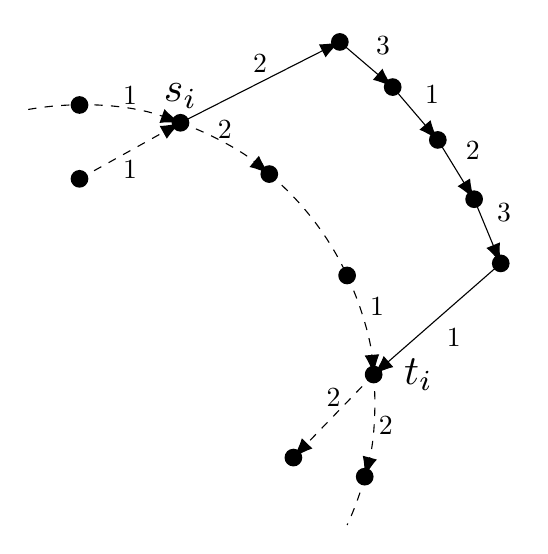
\begin{tikzpicture}[scale=3.75]
					
					\coordinate (V00) at (90:1);
					\coordinate (V01) at (70:1);
					\coordinate (V02) at (5:1);
					\coordinate (V03) at (-15:1);
					\coordinate (V04) at (90:0.75);
					\coordinate (V05) at (-15:0.75);
					%pomiedzy s i t
					\coordinate (V06) at (50:1);
					\coordinate (V07) at (25:1);
					
					\node[scale = 1.5, above ] at (V01) {$s_i$};
					\node[scale = 1.5, right=0.2cm] at (V02) {$t_i$};
					
					\draw[-{Latex[length=2.5mm]}, dashed] (100:1) arc (100:70:1);
					\draw[-{Latex[length=2.5mm]}, dashed] (70:1) arc (70:50:1);
					\draw[ dashed] (50:1) arc (50:25:1);
					\draw[-{Latex[length=2.5mm]}, dashed] (25:1) arc (25:5:1);
					\draw[-{Latex[length=2.5mm]}, dashed] (5:1) arc (5:-15:1);
					\draw[dashed] (-15:1) arc (-15:-25:1);
					
					\foreach \i in {0, 1, 2, 3, 4, 5, 6, 7}
					{
						\path[fill=black] (V0\i) circle (0.03);
					}
					\foreach \i in {1, 2, 3, 4, 5}
					{
						\coordinate (V1\i) at (45 - \i * 360/40 + 360/20:1.5);
						\path[fill=black] (V1\i) circle (0.03);
					}
					\foreach \i/\j in {1/2, 2/3, 3/4, 4/5}
					{
						\path[-{Latex[length=2.5mm]}, draw](V1\i) -- (V1\j);
					}
					\path[-{Latex[length=2.5mm]}, draw](V01) -- (V11);
					\path[-{Latex[length=2.5mm]}, draw](V15) -- (V02);
					
					\path[draw][-{Latex[length=2.5mm]}, dashed] (V04) -- (V01);
					\path[draw][-{Latex[length=2.5mm]}, dashed] (V02) -- (V05);
					\node[above] at ($(V01)!0.5!(V11)$) {$2$};
					\node[above right] at ($(V11)!0.5!(V12)$) {$3$};
					\node[above right] at ($(V12)!0.5!(V13)$) {$1$};
					\node[above right] at ($(V13)!0.5!(V14)$) {$2$};
					\node[above right] at ($(V14)!0.5!(V15)$) {$3$};
					\node[below right] at ($(V15)!0.5!(V02)$) {$1$};
					
					\node[above] at ($(V00)!0.5!(V01)$) {$1$};
					\node[below] at ($(V04)!0.5!(V01)$) {$1$};
					\node[above] at ($(V01)!0.5!(V06)$) {$2$};
					
					\node[right] at ($(V02)!0.5!(V03)$) {$2$};
					\node[above] at ($(V02)!0.5!(V05)$) {$2$};
					\node[above right] at ($(V07)!0.5!(V02)$) {$1$};
					
					
				\end{tikzpicture}

\end{document}